\section{印顺法师科判}
\subsection{四派三系二部一味}
由根本佛教,分成上座與大眾兩部。
上座部東系的一支分別取捨上座及大眾兩部的思想,立足於上座部卻頗同情並吸收大眾部的一部分進步思想,所以成為分別說系。
西系的上座部由於僻處西北印的迦濕彌羅,不與東方接觸,所以發展成為獨立的有部思想;後來內部思想有了歧見,又再分裂。
據大眾部所傳,後來的紅衣(錫蘭銅鍱)部、法藏部、飲光部、化地部、均屬分別說系\footnote{《異部宗輪論》}。
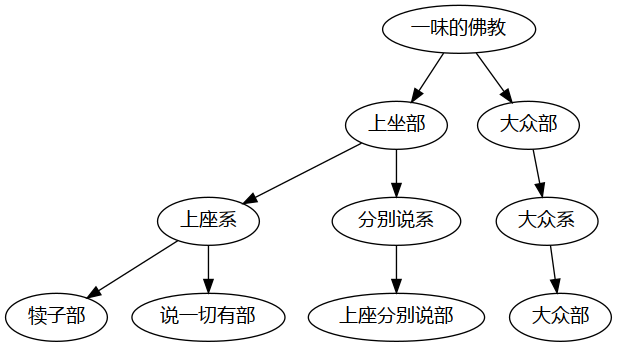
\includegraphics[scale=0.5]{释家/images/四派三系二部一味.png}

\subsection{大乘三系}
\begin{itemize}
  \item 性空唯名
  \item 虚妄唯识
  \item 真常唯心 \footnote{《如來藏經》、《法鼓經》、《大涅槃經》、《勝鬘經》、《不增不減經》、《無上依經》、《楞伽經》、《密嚴經》、《圓覺經》等經,皆屬真常唯心的聖典。後期的密典,十、九亦屬真常唯心。}
\end{itemize}
